\documentclass{article}
\usepackage{amsmath}
\usepackage{tikz}
\usetikzlibrary{matrix}

\begin{document}

\begin{figure}[h]
    \centering
    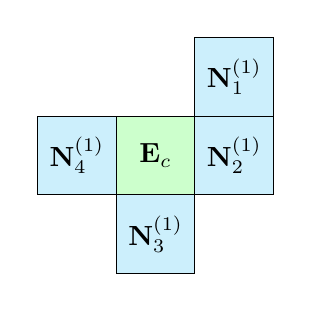
\begin{tikzpicture}
        \matrix (m) [matrix of nodes, nodes={draw, minimum size=1cm, anchor=center}, column sep=-\pgflinewidth, row sep=-\pgflinewidth] {
            & & |[fill=cyan!20]| $\mathbf{N}^{(1)}_{1}$ \\
            |[fill=cyan!20]| $\mathbf{N}^{(1)}_{4}$ & |[fill=green!20]| $\mathbf{E}_{c}$ & |[fill=cyan!20]| $\mathbf{N}^{(1)}_{2}$ \\
            & |[fill=cyan!20]| $\mathbf{N}^{(1)}_{3}$ & \\
        };
    \end{tikzpicture}
    \qquad
    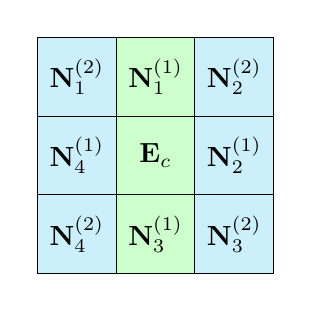
\begin{tikzpicture}
        \matrix (m) [matrix of nodes, nodes={draw, minimum size=1cm, anchor=center}, column sep=-\pgflinewidth, row sep=-\pgflinewidth] {
            |[fill=cyan!20]| $\mathbf{N}^{(2)}_{1}$ & |[fill=green!20]| $\mathbf{N}^{(1)}_{1}$ & |[fill=cyan!20]| $\mathbf{N}^{(2)}_{2}$ \\
            |[fill=cyan!20]| $\mathbf{N}^{(1)}_{4}$ & |[fill=green!20]| $\mathbf{E}_{c}$ & |[fill=cyan!20]| $\mathbf{N}^{(1)}_{2}$ \\
            |[fill=cyan!20]| $\mathbf{N}^{(2)}_{4}$ & |[fill=green!20]| $\mathbf{N}^{(1)}_{3}$ & |[fill=cyan!20]| $\mathbf{N}^{(2)}_{3}$ \\
        };
    \end{tikzpicture}
    
    \caption{Illustrations of our recursive encryption algorithm. There is a two-dimensional plane with $3 \times 3$ pixels, where multiple events $\mathbf{E}_c$ are triggered in the center, and the rest of the pixels are on the mask for synthetic noise. In the $1$st layer of the recursion (left), the algorithm synthesizes the noise $\mathbf{N}^{(1)}_i (i=1,2,3,4)$ in $4$ spatial neighbors horizontally/vertically adjacent to $\mathbf{E}_c$, where $|\mathbf{N}^{(1)}_i| = |\mathbf{E}_c|$. The resulting $\mathbf{N}^{(1)}_i \cup \mathbf{E}_c$ will be the input of the $2$nd layer of the recursion (right). The algorithm, which is blind to $\mathbf{N}^{(1)}_i$ and $\mathbf{E}_c$, synthesizes the noise $\mathbf{N}^{(2)}_i (i=1,2,3,4)$ based on the adjacent events.}
\end{figure}

\end{document}